\documentclass{beamer}

\usefonttheme{professionalfonts} % using non standard fonts for beamer
\usefonttheme{serif} % default family is serif

%\usepackage{hyperref}

%\usepackage{minted}

\usepackage{animate}

\usepackage{graphicx}

\def\Put(#1,#2)#3{\leavevmode\makebox(0,0){\put(#1,#2){#3}}}

\usepackage{color}

\usepackage{tikz}

\usepackage{amssymb}

\usepackage{enumerate}


\newcommand\blfootnote[1]{%

  \begingroup

  \renewcommand\thefootnote{}\footnote{#1}%

  \addtocounter{footnote}{-1}%

  \endgroup

}

\makeatletter

%%%%%%%%%%%%%%%%%%%%%%%%%%%%%% Textclass specific LaTeX commands.

 % this default might be overridden by plain title style

 \newcommand\makebeamertitle{\frame{\maketitle}}%

 % (ERT) argument for the TOC

 \AtBeginDocument{%

   \let\origtableofcontents=\tableofcontents

   \def\tableofcontents{\@ifnextchar[{\origtableofcontents}{\gobbletableofcontents}}

   \def\gobbletableofcontents#1{\origtableofcontents}

 }

%%%%%%%%%%%%%%%%%%%%%%%%%%%%%% User specified LaTeX commands.

\usetheme{Malmoe}

% or ...

\useoutertheme{infolines}

\addtobeamertemplate{headline}{}{\vskip2pt}



\setbeamercovered{transparent}

% or whatever (possibly just delete it)

\makeatother

\begin{document}
\title[DDCEL report]{A Scalable DCEL implementation}
\author[AC]{Andres Calderon}
\institute[Spring'20]{University of California, Riverside}
\makebeamertitle
\newif\iflattersubsect

\AtBeginSection[] {
  \begin{frame}<beamer>
    \frametitle{Outline} 
    \tableofcontents[currentsection]  
  \end{frame}
  \lattersubsectfalse
}

\AtBeginSubsection[] {
  \begin{frame}<beamer>
    \frametitle{Outline} 
    \tableofcontents[currentsubsection]  
  \end{frame}
}

\begin{frame}{Task histogram}{Top 100 tasks by duration\footnote{\tiny{click to enlarge}}...}
  \centering
  \href{https://www.cs.ucr.edu/~acald013/public/RIDIR/figures/TopTasksHist.pdf}{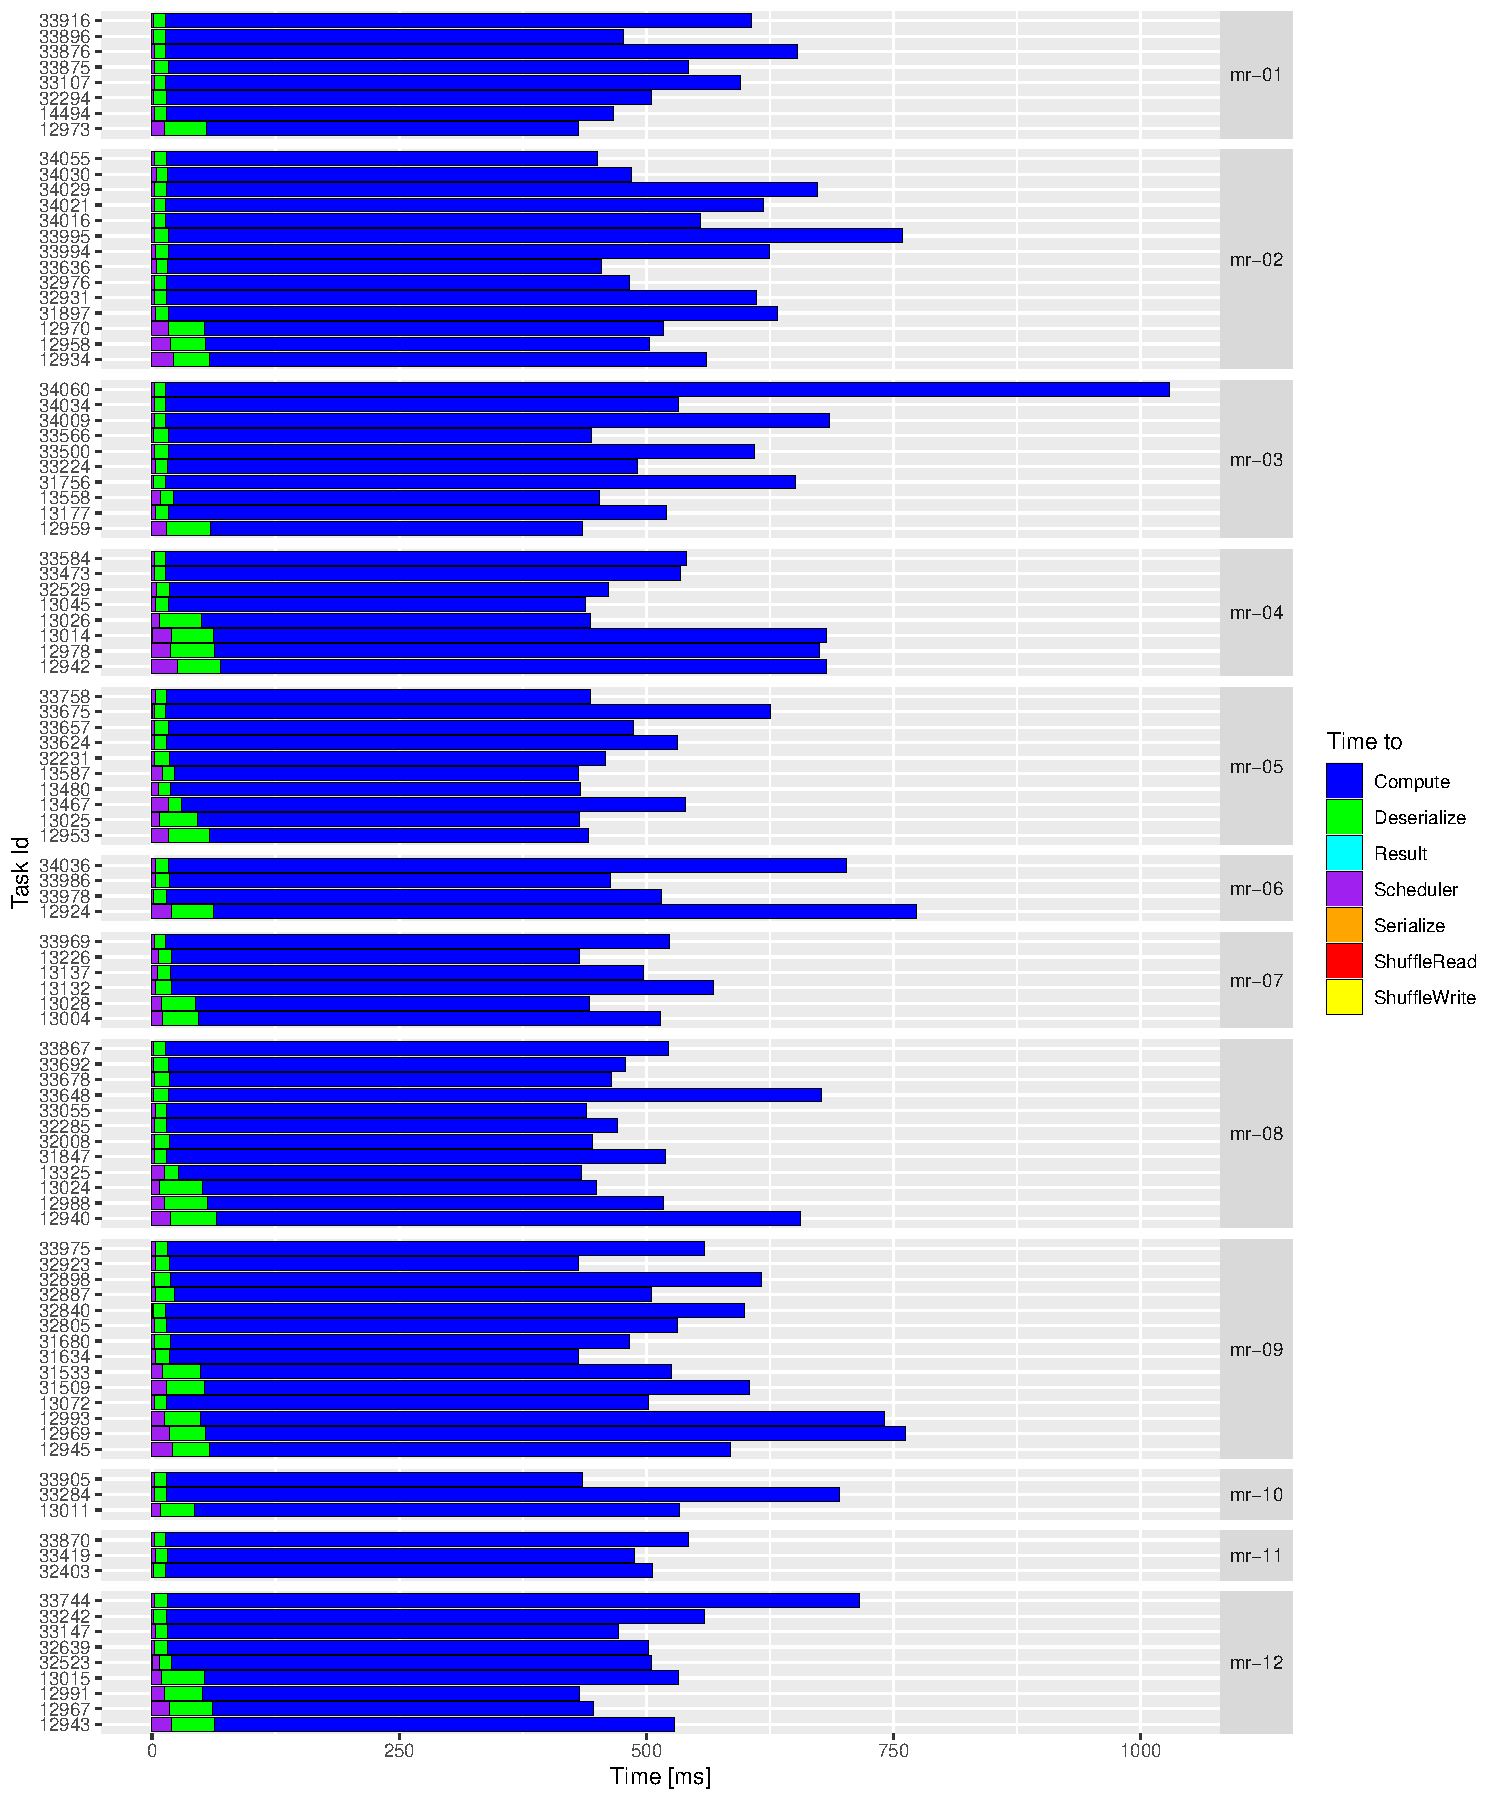
\includegraphics[scale=0.22]{figures/TopTasksHist.pdf}}
\end{frame}

\begin{frame}{Node usage}
  \centering
    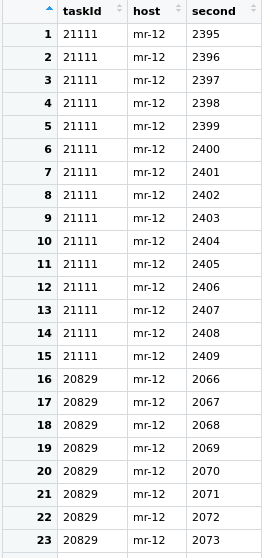
\includegraphics[scale=0.4]{figures/ForPlot}
\end{frame}
\begin{frame}{Node usage}
  \centering
    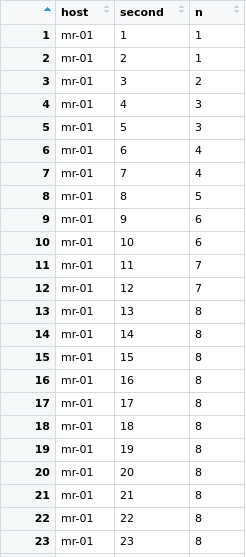
\includegraphics[scale=0.4]{figures/ForPlot2}
\end{frame}

\begin{frame}{Node usage}
    \centering
    \begin{tabular}{l l}
        \hline
                        & n \\ \hline
        Min.         & 1.00\\  
        1st Qu.    & 8.00 \\ 
        Median    & 8.00\\  
        Mean       & 7.81 \\ 
        3rd Qu.    & 8.00 \\
        Max.        &12.00  \\ \hline
    \end{tabular} \\
    \vspace{0.5cm}
    \begin{tabular}{c c c c c c c c c c c c}
    1    & 2    & 3     & 4     & 5     & 6     & 7     & \textbf{8}     & 9    & 10    & 11    & 12 \\
  658   & 362   & 221   & 201   & 147   & 163   & 171 & \textbf{31734}  & 2613   & 163    & 12     & 1 \\ 
    \end{tabular}

\end{frame}

\begin{frame}{What's next}
    \begin{itemize}
        \item Work on the experimental plan
        \item Work on new datasets (in progress)
    \end{itemize}
\end{frame}

\end{document}
